\documentclass[12pt,letterpaper]{article}
\usepackage[utf8]{inputenc}
\usepackage[english]{babel}
\usepackage{amsmath}
\usepackage{amsfonts}
\usepackage{amssymb}
\usepackage{graphicx}
\usepackage[breaklinks=true]{hyperref}
\usepackage[hyphenbreaks]{breakurl}
\usepackage[left=2cm,right=2cm,top=2cm,bottom=2cm]{geometry}
\author{Renee Fatemi, Kim Siang Khaw, Liang Li, Adam Lyon}
\title{Data Production for the Muon g-2 experiment}
\begin{document}

\maketitle

\section{Production Workflow}
This document outlines the workflow of the data production of the Muon g-2 experiment. There are two different production chain: simulation and DAQ. 

\subsection{Simulation production workflow}
Simulation chain involves generating Geant4-based simulated data files, digitization of the truth information and reconstruction of the digitized information. Interaction between the gm2 instance and jobsub and SAM is summarized in Fig. \ref{fig:SimProd}.

\begin{figure}[htbp]
\centering
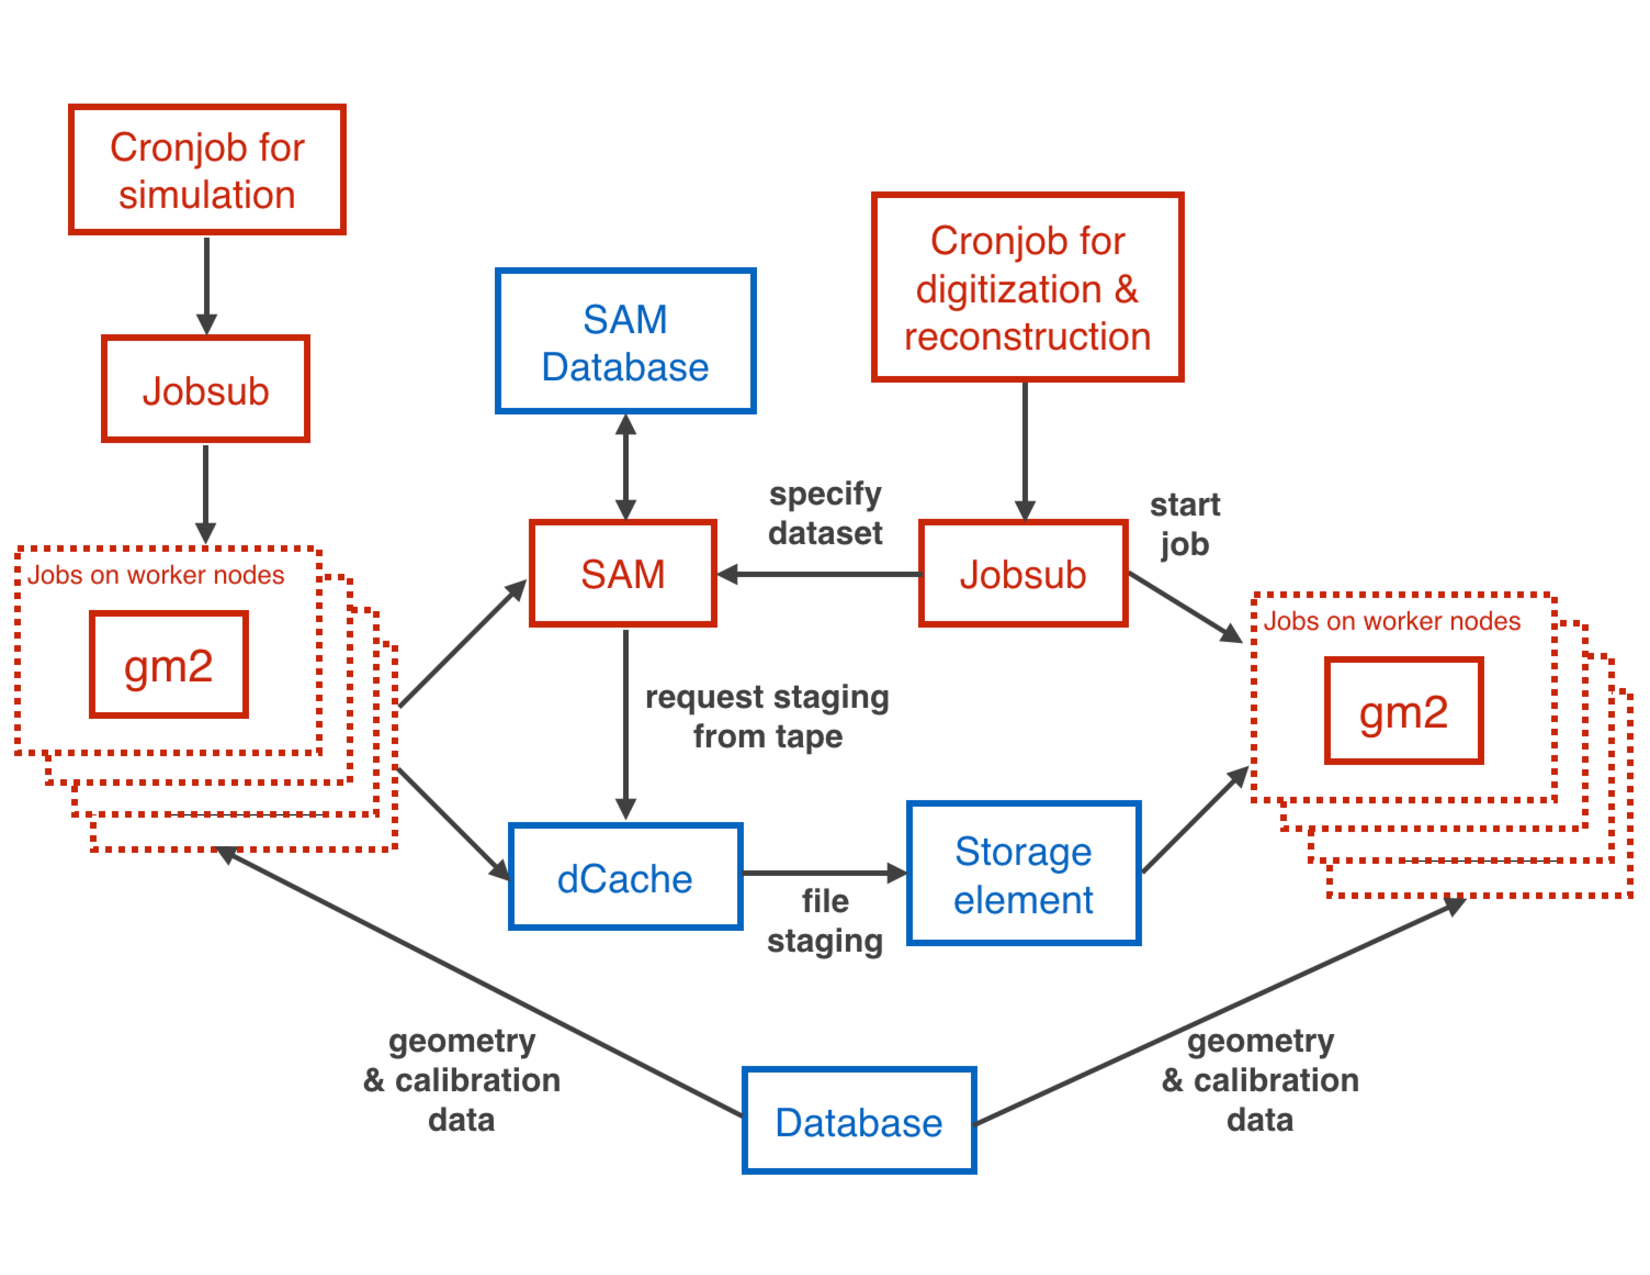
\includegraphics[width=0.7\textwidth]{pics/SimulationProductionWorkflow.pdf} 
\caption{Workflow for the simulation production.}\label{fig:SimProd}
\end{figure}

The following describes the basic steps in the simulation production:

\begin{enumerate}
\item A cronjob is setup to submit jobs to the FNAL grid at a specific time interval.
\item Worker nodes then execute the submitted scripts to generate simulated data. Database may or may not be used for the simulation.
\item Metadata of the generated data files are communicated to SAM data handling system and the files are transferred to FNAL permanent storage area.
\item Another cronjob independent of Cronjob1 is setup to submit jobs to the FNAL to digitize and reconstruct the simulated data.
\item Worker nodes then specify SAM dataset to be digitized and reconstructed.
\item The reconstructed data are then stored in the permanent storage area.
\end{enumerate}

\subsection{DAQ production workflow}

\begin{figure}[htbp]
\centering
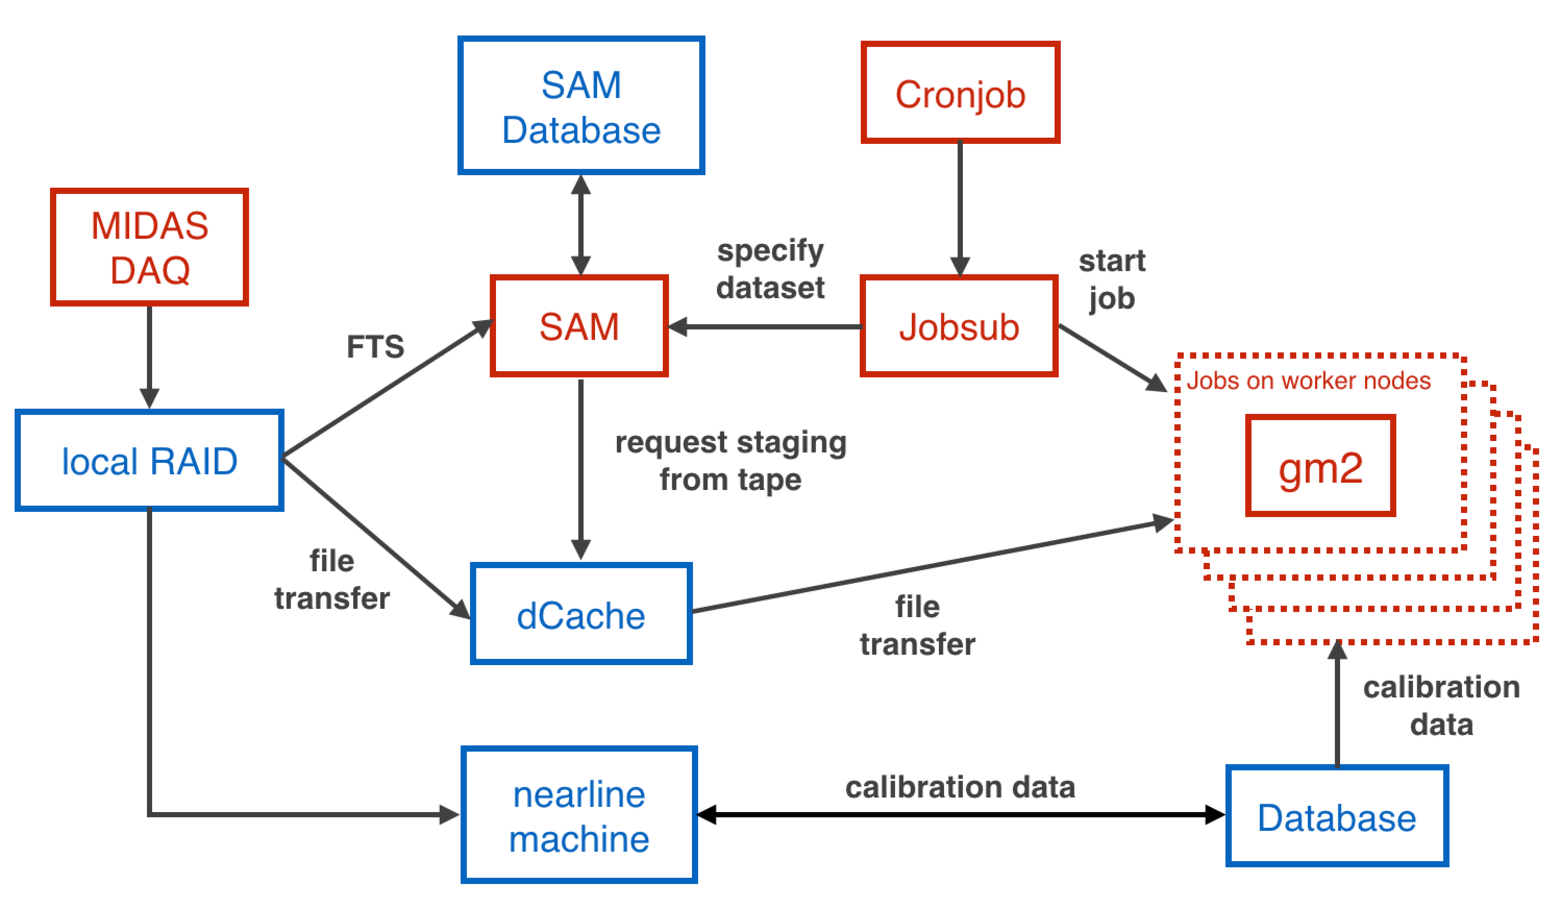
\includegraphics[width=0.7\textwidth]{pics/DAQProductionWorkflow.pdf} 
\caption{Workflow for the DAQ production.}\label{fig:DAQProd}
\end{figure}

The following describes the basic steps in the DAQ production:
\begin{enumerate}
\item MIDAS DAQ outputs raw data and stores them into local RAID storage.
\item A backend machine running FTS transfers raw files to the permanent storage area while communicates with SAM regarding the metadata of the files.
\item At the same time, a nearline machine analyzes specific calibration runs and extracts calibrations from these runs. All the constants are stored in the database.
\item A cronjob is setup to submit jobs to unpack and reconstruct the DAQ data.
\item Worker nodes then specify SAM dataset to be unpacked and reconstructed.
\item The reconstructed data are then stored in the permanent storage area.
\end{enumerate}

\section{SAM Metadata: Metadata definition and dataset definition}
How to insert metadata using FTS, art, etc. What are the metadata we want to insert, etc.

\section{Workflow of the data production: Implementation }
mock data handling, type of runs, working schedule, deadlines, etc

\section{Versioning of the scripts/codes (related to releases)}

\section{POMS: What do we know so far}
Reference slides:

\url{https://indico.fnal.gov/getFile.py/access?contribId=8&resId=0&materialId=slides&confId=12120}

\end{document}